\documentclass[tikz,border=8pt]{standalone}
% Shared look for every TikZ diagram. Load with \input{../../tools/tikz-style.tex}
\usepackage[T1]{fontenc}
\usepackage{lmodern}
\renewcommand{\sfdefault}{lmr}  % diagrams use the same serif as the text
\usetikzlibrary{arrows.meta, positioning, shapes.geometric, calc, fit, backgrounds}
\definecolor{cblue}{HTML}{4C78A8}
\definecolor{corange}{HTML}{F58518}
\definecolor{cgreen}{HTML}{54A24B}
\definecolor{cred}{HTML}{E45756}
\definecolor{cpurple}{HTML}{B279A2}
\definecolor{cgrey}{HTML}{6B6B6B}
\tikzset{
  every picture/.style={font=\sffamily, line width=1.2pt},
  box/.style={draw=#1, fill=#1!12, rounded corners=4pt, align=center, inner sep=7pt, minimum height=1.1cm},
  box/.default=cgrey,
  arrow/.style={-{Stealth[length=3mm]}, draw=cgrey, line width=1.4pt},
  title/.style={font=\sffamily\bfseries\Large},
  note/.style={font=\sffamily\small, text=cgrey, align=center},
}
\AtBeginDocument{\hyphenpenalty=10000 \exhyphenpenalty=10000}

% Inverse kinematics example: wanted v = 0.3 m/s, omega = 0.5 rad/s, so the robot drives a circle of radius
% R = v / omega = 0.6 m. The outer (right) wheel, at R + L/2 = 0.7 m, needs 0.35 m/s; the inner (left) wheel,
% at R - L/2 = 0.5 m, needs 0.25 m/s. Arrow lengths are drawn in proportion.
\begin{document}
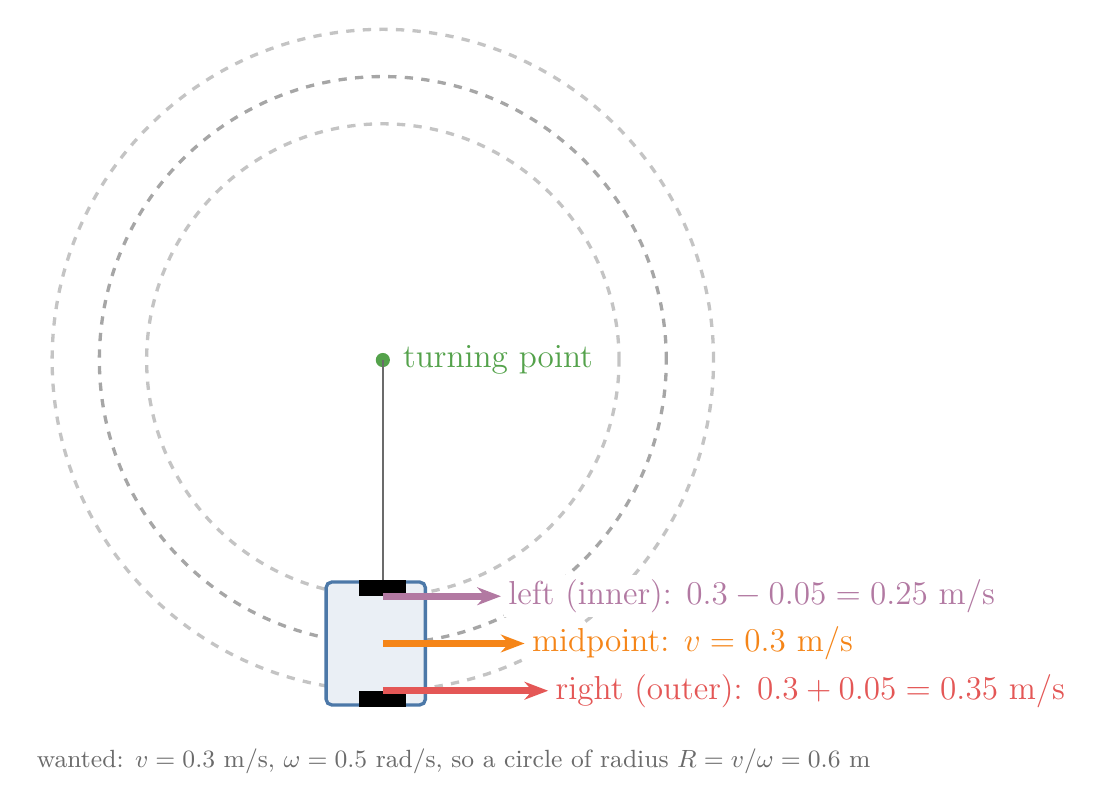
\begin{tikzpicture}[scale=6, every node/.append style={font=\large}]
  \coordinate (C) at (0,0.6);
  \draw[cgrey!60, dashed] (C) circle (0.6);
  \draw[cgrey!40, dashed] (C) circle (0.7); \draw[cgrey!40, dashed] (C) circle (0.5);
  \fill[cgreen] (C) circle (0.015); \node[cgreen, right] at (0.02,0.6) {turning point};
  \draw[cgrey, line width=0.8pt] (0,0.6) -- (0,-0.12);
  \draw[cblue, fill=cblue!12, rounded corners=2pt] (-0.12,-0.13) rectangle (0.09,0.13);
  \fill[black] (-0.05,0.1) rectangle (0.05,0.135); \fill[black] (-0.05,-0.135) rectangle (0.05,-0.1);
  \draw[-{Stealth[length=3mm]}, cred, line width=2.4pt] (0,-0.1) -- (0.35,-0.1) node[right, fill=white, inner sep=1.5pt] {right (outer): $0.3 + 0.05 = 0.35$ m/s};
  \draw[-{Stealth[length=3mm]}, corange, line width=2.4pt] (0,0) -- (0.30,0) node[right, fill=white, inner sep=1.5pt] {midpoint: $v = 0.3$ m/s};
  \draw[-{Stealth[length=3mm]}, cpurple, line width=2.4pt] (0,0.1) -- (0.25,0.1) node[right, fill=white, inner sep=1.5pt] {left (inner): $0.3 - 0.05 = 0.25$ m/s};
  \node[note, anchor=north] at (0.15,-0.2) {wanted: $v = 0.3$ m/s, $\omega = 0.5$ rad/s, so a circle of radius $R = v / \omega = 0.6$ m};
\end{tikzpicture}
\end{document}
